\documentclass[dvipsnames,parskip,a4paper]{scrartcl}

% color and design packages
\usepackage[usenames,dvipsnames]{xcolor}
\usepackage{tikz}
\usetikzlibrary{positioning}

\usepackage{pifont}
\usepackage{graphicx}
\usepackage{etoolbox}
\usepackage{longtable}
\usepackage{fontspec}
\usepackage[export]{adjustbox}
\usepackage[utf8]{inputenc}
\usepackage[margin=1.5cm]{geometry}
\usepackage{nopageno}
\usepackage{titling}

\setlength{\parskip}{0pt}
\setlength{\tabcolsep}{0pt}

% clear date
\predate{}
\postdate{}
\date{}

\title{Elemental Dice}
\author{Emil Indzhev}

% Our consistent sizing
\newcommand{\cardroundingradius}{4mm}
\newcommand{\cardboxroundingradius}{0.5mm}
\newcommand{\cardtextborderspace}{1.28mm}
\newcommand{\cardwidth}{57.5mm}
\newcommand{\cardheight}{89mm}
\newcommand{\cardtitleheight}{7.1mm}
\newcommand{\cardtextheight}{15.8mm}
\newcommand{\cardtcheight}{6mm}
\newcommand{\cardborderspace}{3mm}
\newcommand{\cardvspace}{2.5mm}

\newcommand{\iconsize}{3.4mm}
\newcommand{\icondepth}{0.45mm}

\newcommand{\cardimgborderspace}{0.1mm}
\newcommand{\cardimgwidth}{51.3mm}
\newcommand{\cardimgheight}{46.4mm}
\newcommand{\cardimghalfwidth}{25.65mm}
\newcommand{\cardimghalfheight}{23.2mm}

% Consistent colors
\newcommand{\cardcolor}{gray!60}
\newcommand{\cardboxcolor}{gray!30}
\newcommand{\cardboxbordercolor}{gray}
\newcommand{\cardbordercolor}{gray}

% Card template
\newcommand{\card}[5]{

\begin{tikzpicture}[baseline = (current bounding box.center)]
\draw[rounded corners = \cardroundingradius, fill = \cardcolor, draw = \cardbordercolor, thick] (0,0) rectangle
    (\cardwidth, \cardheight);

\node (title) at (0.5 * \cardwidth, \cardheight - \cardborderspace)
    [ anchor = north, fill = \cardboxcolor, draw = \cardboxbordercolor, thick, text centered, 
    rounded corners = \cardboxroundingradius,
    inner sep = \cardtextborderspace,
    text width = \cardwidth - 2 * (\cardborderspace + \cardtextborderspace),
    minimum height = \cardtitleheight]
    { \Large #1 };

\node (image) at (0.5 * \cardwidth, \cardborderspace + \cardtcheight + \cardtextheight + 2 * \cardvspace)
    [ anchor = south, fill = \cardboxcolor, thick, text centered,
    rounded corners = \cardboxroundingradius,
    inner sep = \cardimgborderspace,
    text width = \cardwidth - 2 * (\cardborderspace + \cardimgborderspace),
    minimum height = \cardheight - \cardtcheight - \cardtextheight - \cardtitleheight - 2 * \cardborderspace - 3 * \cardvspace]
    {\includegraphics[max size={\cardimgwidth}{\cardimgheight}, min size={\cardimgwidth}{\cardimgheight}, Clip*={.5\width-\cardimghalfwidth} {.5\height-\cardimghalfheight} {.5\width+\cardimghalfwidth} {.5\height+\cardimghalfheight}]{ #5 }};

\node (image_border) at (0.5 * \cardwidth, \cardborderspace + \cardtcheight + \cardtextheight + 2 * \cardvspace)
    [ anchor = south, draw = \cardboxbordercolor, thick, text centered,
    rounded corners = \cardboxroundingradius,
    inner sep = \cardimgborderspace,
    text width = \cardwidth - 2 * (\cardborderspace + \cardimgborderspace),
    minimum height = \cardheight - \cardtcheight - \cardtextheight - \cardtitleheight - 2 * \cardborderspace - 3 * \cardvspace]
    {};

\node (text) at (0.5 * \cardwidth, \cardborderspace + \cardtcheight + \cardvspace)
    [ anchor = south, fill = \cardboxcolor, draw = \cardboxbordercolor, thick, text centered,
    rounded corners = \cardboxroundingradius,
    inner sep = \cardtextborderspace,
    text width = \cardwidth - 2 * (\cardborderspace + \cardtextborderspace),
    minimum height = \cardtextheight]
    { #3 };

\node (type)
    [ fill = \cardboxcolor, draw = \cardboxbordercolor, thick,
    below left = \cardvspace + \cardtcheight and 0mm of text, anchor = south west,
    rounded corners = \cardboxroundingradius,
    inner sep = \cardtextborderspace,
    minimum height = \cardtcheight]
    { #2 };

\node (cost)
    [ fill = \cardboxcolor, draw = \cardboxbordercolor, thick,
    below right = \cardvspace + \cardtcheight and 0mm of text, anchor = south east,
    rounded corners = \cardboxroundingradius,
    inner sep = \cardtextborderspace,
    minimum height = \cardtcheight]
    { #4 };

\end{tikzpicture}%

}

% Elemental symbols
\newcommand{\icon}[1]{\raisebox{-\icondepth}{\includegraphics[height=\iconsize]{ #1 }}}
\newcommand{\fire}{\icon{icons/fire.png}}
\newcommand{\earth}{\icon{icons/earth.png}}
\newcommand{\water}{\icon{icons/water.png}}
\newcommand{\nature}{\icon{icons/nature.png}}
\newcommand{\magic}{\icon{icons/magic.png}}
\newcommand{\gold}{\icon{icons/gold.png}}
\newcommand{\chance}{\icon{icons/chance.png}}

% Costs
\newcommand{\starter}{Starter}
\newcommand{\draft}{Draft}
\newcommand{\onecost}{3 gold}
\newcommand{\twocost}{6 gold}
\newcommand{\threecost}{10 gold}
\newcommand{\fourcost}{15 gold}
\newcommand{\fivecost}{21 gold}

\newcommand{\facedowncost}{2}
\newcommand{\refreshcost}{2}
\newcommand{\refreshcostincrease}{1}
\newcommand{\expresscost}{3}

\newcommand{\startgold}{5}

\newcommand{\handsize}{4}
\newcommand{\dacedownsize}{2}
\newcommand{\shopsize}{5}

\newcommand{\starthp}{90}
\newcommand{\maxhp}{160}

\begin{document}

\maketitle

\newpage

\subsection*{Summary}

The game is played between two players who build their decks and take turns playing cards from them. Their decks start weak, but they can improve them by buying better cards or removing weak ones. Each player also has some mana (used to play cards), gold (used to buy cards) and HP (if it reaches 0, the player loses). Some cards give gold, deal damage or restore HP, while others provide various forms of utility, shielding or buffs. Seven elemental dice determine the strengths of various cards: Fire \fire, Earth \earth, Water \water, Nature \nature, Gold \gold, Magic \magic \ and Chance \chance. They are rolled at the start and stay like that. However, some cards can change the values of these dice, thus changing how strong other cards are.

\subsection*{Win condition}

The game ends in one of two cases:

\begin{itemize}
\item A player's HP reaches 0 (or less). Then the other player wins. If both players' HPs reach 0 at the same time, the one whose card caused this wins.
\item A player's HP reaches \maxhp \ (or more). Then they win. (Cannot happen to both players simultaneously.)
\end{itemize}

\subsection*{The cards}

There are some \starter \ and \draft \ cards, which each player's deck starts with. The rest are buyable from the shop (explained later) and have gold costs: \onecost, \twocost, \threecost, \fourcost \ or \fivecost.

\vspace{4pt}

Mechanically, there are 3 types of cards:

\begin{itemize}
\item Spell -- The most common type; these cards get played from a player's hand and cost 1 mana to play (default a player only gets 1 mana per turn and, if unused, it is lost at the end of the turn).
\item Blessing -- Similar to a spell, except that they cost no mana (so any number of them can be played per turn) and that they can also be played during the opponent's turn.
\item Relic -- These cards are deployed immediately upon being acquired and remain in play until the end of the game (i.e. they provide passive effects).
\end{itemize}

Spells and blessings are usually played from the hand, but can also be placed face down and then later played like a blessing, i.e. for no mana and potentially during the opponent's turn (explained later).

\vspace{4pt}

We can also classify most cards depending on what they do:

\begin{itemize}
\item Attack -- ``Deal X damage'' cards (i.e. reduce the opponent's HP). They all scale with one or two of \fire, \earth, \water, \chance \ and \magic. Attacks that scale with \water \ deal damage to both players.
\item Restore -- ``Restore X HP'' cards. They all scale with \nature \ and possibly one of the attack elements.
\item Gold -- ``Gain X gold'' cards. They all (except the starter cards) scale with \gold \ and possibly one of the attack elements.
\item Buff -- ``Double the strength of all your cards that scale with X'' cards. They buff other cards.
\item Shield -- ``Shield X against incoming damage that scales with Y'' cards. They reduce incoming damage.
\item Dice Control -- various cards that affect the dice (either changing their values or rerolling them). These are the only way to change the dice values (and thus affect how strong various other cards are).
\item Draw -- ``Draw X cards'' cards. Useful for finding the valuable cards.
\item Mana -- ``Gain X mana'' cards. Useful for playing multiple spells in a single turn.
\item Removal -- ``Permanently remove X cards from ...'' cards. Permanently removing a card means removing it from one's deck and moving it to the removed cards pile. Useful for removing bad cards.
\item Other utility -- various other cards with hard to categorize effects. Some may allow seeing otherwise hidden information or messing with the opponent in some way, etc.
\end{itemize}

\subsection*{Elemental scaling}

Many cards' descriptions have an element symbol instead of a number, e.g. ``Deal \fire \ damage to your opponent''. This means that the amount of damage dealt is equal to the current value of the \fire \ die. We say that this card scales with \fire. Note that the die is not rerolled when playing such a card.

\vspace{4pt}

It is also possible to have a stronger scaling like 2\hspace{1pt}$\times$\hspace{1pt}\fire, which would mean that the damage is equal to 2 times the current value of the \fire \ die. Other cards may scale with multiple elements like \earth\hspace{1pt}$+$\hspace{1pt}\chance \ or \water\hspace{1pt}\times\hspace{1pt}\magic, which would mean that the damage is equal to sum or product, respectively, of the current values of the two listed dice.

\vspace{4pt}

In all multi-element scaling cards, the combination is a sum, if neither element is \magic, and a product, otherwise. There are no single-element \magic \ scaling cards, i.e. \magic \ is always a multiplier.

\vspace{4pt}

\subsection*{The \chance \ die}

Unlike all other dice, whenever its value is needed by a card that scales with it, it is rerolled before executing (and calculating the strength of) the card. Note that dice control cards may still affect the \chance \ die, though this usually achieves nothing.

\subsection*{Buffs}

Buffs (``Double the strength of all your cards that scale with X until the end of your turn.'') work by doubling the effective values of all dice except \magic \ in the strentgh calculations for all cards (of the player with the buff) that scale with X (and possibly something else). Multiple buffs may affect the same cards (e.g. two buffs means times 4). Buffs are discarded at the end of the player's turn (i.e., if played during the opponent's turn, a buff lasts through that and the player's turn.)

\vspace{4pt}

Example: Alice plays buff that targets \fire. She then plays a \fire\hspace{1pt}$\times$\hspace{1pt}\magic \ attack, a \nature\hspace{1pt}$+$\hspace{1pt}\fire \ restore and a \water\hspace{1pt}$+$\hspace{1pt}\earth \ attack. The first two will be doubled (i.e. will do 2\hspace{1pt}$\times$\hspace{1pt}\fire\hspace{1pt}$\times$\hspace{1pt}\magic \ damage and 2\hspace{1pt}$\times$\hspace{1pt}\nature\hspace{1pt}$+$\hspace{1pt}2\hspace{1pt}$\times$\hspace{1pt}\fire \ restoration, respectively), while the last attack will not be doubled.

\subsection*{Shields}

Shields (``Shield X against incoming damage that scales with Y until the end of your opponent's turn'') work by subtracting (without going negative) the value of die X from all dice except \magic \ in the strentgh calculations for all incoming damage (towards the player with the shielf) that scales with X (and possibly something else). Multiple shields may affect the same card. Shields are discarded at the end of the opponent's turn (i.e., if played during the player's turn, a shield lasts through that and the opponent's turn.)

\vspace{4pt}

This shield subtraction happens after the doubling due to buffs. Both the shield and/or the incoming damage may be buffed. In the first case, the substracted value is doubled. In the second case, the value(s) being subtracted from is/are doubled.

\vspace{4pt}

Example: During her turn, Alice plays a \fire \ buff and a 2\hspace{1pt}$\times$\hspace{1pt}\fire \ attack. The value of the \fire \ die is 4, so this attack would deal $2 \times 2 \times 4 = 16$ damage. However, Bob counters by playing a \water \ shield against \fire. The value of the \water \ die is 3, so the attack now deals $2 \times (2 \times 4 - 3) = 10$ damage. Had Bob also played a \water \ buff, the attack would have dealt $2 \times (2 \times 4 - 2 \times 3) = 4$.

\vspace{4pt}

Example 2: Alice plays a \water\hspace{1pt}$+$\hspace{1pt}\earth \ attack that targets both players. The value of the \water \ die is 2 and that of the \earth \ one is 5, so this attack would deal $2 + 5 = 7$ damage to both players. However, Bob counters by playing a ``Magical Barrier''. The value of the \magic \ die is 4. The attack now deals $0 + (5 - 4) = 1$ damage to Bob (since $2 - 4$ is negative) and still 5 damage to Alice.

\subsection*{Gold}

Gold (represented by the coins) is gained passively (1 per turn) and by playing cards. Other than with gold cards: A player dealing damage or restoring HP (to their opponent or themselves) receives gold equal to half the damage dealt/HP restored (rounded up). Note that, if a card deals damage to both players, the gold gained is half of the total damage dealt. Gold is mainly spent on refreshing the shop, buying cards or placing face down cards.

\subsection*{Initial setup}

\begin{itemize}
\item Each player starts with \starthp \ HP (out of \maxhp) and \startgold \ gold.
\item All seven elemental dice are rolled and ordered next to the HP tracker like so: \fire, \earth, \water, \nature, \gold, \magic, \chance.
\item All cards with gold costs are shuffled together and form the shop's draw pile. No shop cards are laid out at the start.
\item The 8 \draft \ cards (``Fire'', ``Tremor'', ``Heavy Rain'', ``Blind Attack'', ``Flower Gardens'', ``Marketplace'', ``Gambling'' and ``Cheap Trick'') are shuffled together; 6 of them are dealt out and the other 2 are permanently removed.
\item Each player rolls a die and whoever rolls higher choses who goes first. (In case of a tie, reroll.)
\item The player who rolled lower in the first player determination may decide to swap who goes first and who goes second by offering 1 advantage (ability to change a die by 1) to the other player. If this happens, the other player has the same option, but for 2 advantage. This repeats (with increasing advantage numbers) until one player passes up on using this option. Only the final advantage offer remains in effect, as this is effectively an auction for the turn order.
\item The first player drafts (chooses) 1 of the dealt out \draft \ cards, the second one drafts 2 of the remaining ones, the first one drafts 2, and the last card goes to the second player.
\item The starting draw pile of each player is formed by shuffling together the 9 Starter cards (8 ``Basic Income'' and 1 ``Lucky Find'') and their 3 chosen \draft \ cards.
\item The player with X advantage (if any) may change the value of a die by 1 up to X times (may be the same die, different dice or any other combination).
\item Each player draws \handsize \ cards from their draw pile into their hand and the first player starts their turn.
\end{itemize}

\subsection*{A player's turn}

At the start of their turn, the player gains 1 gold and 1 mana. After that they may do any of the following actions (in any order, possibly multiple times and/or interleaved):

\begin{itemize}
\item Play a spell from their hand at the cost of 1 mana.
\item Play a blessing from their hand at no cost.
\item Place a face down card at the cost of 1 mana and \facedowncost \ gold. A player may have at most \dacedownsize \ face down cards at a time.
\item Play (flip over and activate) any number of face down cards at no cost.
\item Refresh the shop. The first refresh in a turn costs \refreshcost \ gold and each subsequent is \refreshcostincrease \ gold more expensive.
Refreshing the shop consists of moving the currently laid out shop cards (if any) to the shop's discard pile followed by drawing and laying out \shopsize \ cards from the shop's draw pile. Note that initially there are no shop cards laid out.
\item Buy a card from the laid out shop cards by paying its cost. May be done at most once per turn.
The bought card is not replaced, so the shop can become empty again. The bought card goes to the player's discard pile, unless it is relic, in which case it is immediately and permanently deployed.
\end{itemize}

Whenever a card is played it is kept in the player's play area until the end of their turn (after which it is discarded). Cards whose effect lasts longer (e.g. buffs and shields) are kept in the play area until their effect expires (at which point they are discarded).

\vspace{4pt}

After the player's turn is over, they lose all their mana, discard their entire hand and their played cards (unless still active) and then draw \handsize \ cards from their draw pile.

\subsection*{Shop Summary}

The shop is where cards are bought from. It has its own draw and discard piles and a laid out shop. Initially, all buyable cards are shuffled in its draw pile and no cards are laid out. Then, by paying some gold, players may refresh the shop -- discard all laid out cards and then draw and lay out \shopsize \ cards. Cards may only be bought from the laid out shop (happens by paying their gold cost).

\subsection*{Interruptions from the opponent}

Whenever the current player plays a spell that scales with an element/elements (i.e. an attack, a restore or a gold card), the opponent can interrupt it before it is executed (rolling the \chance \ die due to its rule is considered part of the execution). The interrupted card is rotated by 90 degrees clockwise to indicate that it is yet to be executed. Then the opponent can play any number of cards (which can only be face down cards or blessings from their hand, since it is not their turn). After they declare that they are done the current player has the chance to do the same (though, since it is their turn, they can do any valid action: play spells from their hand, place face down cards or even interract with the shop). This can repeat any number of times (i.e. the opponent going again, then the current player, etc.) until one of the players chooses to do nothing (i.e. passes). After that the interrupted card is executed (and rotated by 90 degrees counterclockwise) and the current player continues their regular turn.

\vspace{4pt}

If either player plays another elemental spell during this process, the other player can interrupt it, too. In that case, this process starts again for that card. When a player passes and the process ends, the last interrupted card is resolved. After that the player whose card that was can continue playing cards (or other valid for them actions) and so on until the previous interrupted card is resolved. Finally, when the first interrupted card is resolved, the whole thing ends. Note that it is important to keep track of the order of the interrupted cards, so consider laying them out in a time line, if needed.

\vspace{4pt}

The opponent has one more opportunity to interrupt during the current player's turn: right after the start (after the current player gets his gold and mana, but before doing any actions). All the same rules apply, except that there is no initial interrupted card, so after the interruption process is done, the current player simply starts their turn.

\vspace{4pt}

All cards played by the opponent (unless still active) are discarded at the end of the current player's turn.

\vspace{4pt}

Example: In a very close game, Alice is at 4 HP and Bob at 2 HP. During her turn, Alice plays a \fire \ attack. The current value of \fire \ is 6, so she would win. Bob interrupts this and plays a face down card that allows him to reroll the \fire \ die. It rolls a 2, so he is still losing. Then, he plays a blessing from his hand: a \water \ shield against \fire \ attacks. The value of \water \ is 4, so this would mitigate all damage. He is done for now. Alice then plays a blessing that gives her mana, allowing her to play another spell (from her hand): ``Trickster God'', which she uses to swap the values of the \fire \ and \water \ dice. Bob is again losing so he plays his second face down card: a \chance \ attack, which has a 50\% chance of winning him the game. Alice interrupts this by playing a \gold \ shield against single element attacks. The value of \gold \ is 2, so Bob needs a 6 to win. Alice is done and Bob passes as he has nothing more to do. He rolls the \chace \ die to execute his attack, but the die rolls a 4. He is done and Alice passes, as she is winning anyway. Finally, Alice's attack is executed and she wins the game.

\subsection*{Discard pile}

Whenever a player needs to discard some number of cards (from their hand or face down cards), but has fewer than that, they simply discard all such cards and that effect is considered as executed. Instead, if the player has more cards than that, they chose which cards to discard.

\vspace*{4pt}

Whenever a card needs to be drawn from a deck's draw pile, but it is empty, its discard pile is shuffled and it becomes the draw pile. This is never triggered by effects without the ``draw'' keyword (e.g. ``Look at top X cards of your draw pile'', even if the draw pile has fewer than X cards).

\subsection*{Private and public information}

A player's hand, face down cards, discard pile and discards are private information, i.e. only they may see them. The laid out shop, the shop's discard pile, the removed cards pile, a player's played cards, bought cards, removed cards, gold, HP, mana and all counts (e.g. number of cards in hand) are all public information, i.e. everyone can see them. All draw piles are hidden information, i.e. nobody can see them.

\subsection*{Trackers and tokens}

Use the 7 colored dice for the elements. Use the spare dice to roll for turn order choice. Use the HP tracker (the large grid) and the two differently colored pawns to keep track of players' HPs. Use the coins to keep track of players' gold. If needed, use the spare dice or other tokens to keep track of mana.

\subsection*{Resigning}

This is a two player game that is played until one player wins and the other loses. If at any point, during their turn, a player no longer wishes to continue (since they are convinced that they cannot win anymore or any other reason), they can resign. This means they lose the game and their opponent wins. This is a full-fledged victory. However, resigning too easily is discouraged. Resigning right before one's opponent is about to pull off a big combo and win is also discouraged. In general, players should try their best to play games out until the end.

\subsection*{Card Clarifications}

\begin{itemize}
\item ``Second Chance'', ``Sleight of Hand'', ``Calculated Risk'' and ``Smoke and Mirrors'' affect only one die (chosen by the player), i.e. their effects cannot be split up over multiple dice.
\item ``Wish'' (``Buy any unowned card in the game for free, then shuffle the shop's draw pile.'') can target the shop and its draw and discard piles. The chosen card is public information.
\item ``At What Cost'' (``Permanently remove a relic you own upon buying this; gain 1 extra mana at the start of your turn.'') cannot be bought, if the player does not own another relic card.
\item ``Veto'' (``Your opponent receives 1 less mana at the start of their next turn.'') is discarded at the start of the opponent's next turn (i.e. after the player has drawn their hand at the end of their turn).
\item ``Madness'' (``Upon buying this reroll all dice and permanently remove this card.'') counts as being played for the purposes of other cards (e.g. ``Truly Blessed'')
\end{itemize}

\newpage

% HP tracker
\begin{tikzpicture}[overlay,remember picture]
\begin{scope}[shift=(current page.center)]
    % Define the grid size
    \def\rows{16}
    \def\cols{10}
    \def\cellsize{16.68mm}
    
    % Calculate the total width and height of the grid
    \def\gridwidth{\cols*\cellsize}
    \def\gridheight{\rows*\cellsize}
    
    % Draw the grid
    \draw[step=\cellsize] (-0.5*\gridwidth, -0.5*\gridheight) grid (0.5*\gridwidth, 0.5*\gridheight);
    
    \foreach \y in {15,...,0}
        \foreach \x in {1,...,10}
            \pgfmathsetmacro\z{int(\x+(10*\y))}
            \node at (-0.5*\gridwidth+\x*\cellsize-\cellsize/2,-0.5*\gridheight+\y*\cellsize+\cellsize/2) {\z};

\end{scope}
\end{tikzpicture}    

\newpage

\begin{longtable}{ c c c }

\card{Fire}{Spell}{Deal \fire \ damage to your opponent.}{\draft}{imgs/fire.png}
&
\card{Tremor}{Spell}{Deal \earth \ damage to your opponent.}{\draft}{imgs/tremor.png}
&
\card{Heavy Rain}{Spell}{Deal \water \ damage to both yourself and  your opponent.}{\draft}{imgs/heavy_rain.png}
&
\card{Blind Attack}{Spell}{Deal \chance \ damage to your opponent.}{\draft}{imgs/blind_attack.png}
&
\card{Blazing Fire}{Spell}{Deal 2\hspace{1pt}$\times$\hspace{1pt}\fire \ damage to your opponent.}{\threecost}{imgs/blazing_fire.png}
&
\card{Massive Earthquake}{Spell}{Deal 2\hspace{1pt}$\times$\hspace{1pt}\earth \ damage to your opponent.}{\threecost}{imgs/massive_earthquake.png}
&
\card{Torrential Rainstorm}{Spell}{Deal 2\hspace{1pt}$\times$\hspace{1pt}\water \ damage to both yourself and your opponent.}{\threecost}{imgs/torrential_rainstorm.png}
&
\card{Haphazard Offence}{Spell}{Deal 2\hspace{1pt}$\times$\hspace{1pt}\chance \ to your opponent.}{\threecost}{imgs/haphazard_offence.png}
&
\card{Lava Surge}{Spell}{Deal \fire\hspace{1pt}$+$\hspace{1pt}\earth \ damage to your opponent.}{\threecost}{imgs/lava_surge.png}
&
\card{Erratic Blaze}{Spell}{Deal \fire\hspace{1pt}$+$\hspace{1pt}\chance \ damage to your opponent.}{\threecost}{imgs/erratic_blaze.png}
&
\card{Chaotic Avalanche}{Spell}{Deal \earth\hspace{1pt}$+$\hspace{1pt}\chance \ damage to your opponent.}{\threecost}{imgs/chaotic_avalanche.png}
&
\card{Scalding Fog}{Spell}{Deal \water\hspace{1pt}$+$\hspace{1pt}\fire \ damage to both yourself and your opponent.}{\threecost}{imgs/scalding_fog.png}
&
\card{Devastating Mudslide}{Spell}{Deal \water\hspace{1pt}$+$\hspace{1pt}\earth \ damage to both yourself and your opponent.}{\threecost}{imgs/devastating_mudslide.png}
&
\card{Wild Seas}{Spell}{Deal \water\hspace{1pt}$+$\hspace{1pt}\chance \ damage to both yourself and your opponent.}{\threecost}{imgs/wild_seas.png}
&
\card{Magical Inferno}{Spell}{Deal \fire\hspace{1pt}$\times$\hspace{1pt}\magic \ damage to your opponent.}{\fourcost}{imgs/magical_inferno.png}
&
\card{Arcane Meteor}{Spell}{Deal \earth\hspace{1pt}$\times$\hspace{1pt}\magic \ damage to your opponent.}{\fourcost}{imgs/arcane_meteor.png}
&
\card{Biblical Flood}{Spell}{Deal \water\hspace{1pt}$\times$\hspace{1pt}\magic \ damage to both yourself and your opponent.}{\fourcost}{imgs/biblical_flood.png}
&
\card{Ethereal Havoc}{Spell}{Deal \chance\hspace{1pt}$\times$\hspace{1pt}\magic \ damage to your opponent.}{\fourcost}{imgs/ethereal_havoc.png}
&

\card{Flower Gardens}{Spell}{Restore \nature \ HP.}{\draft}{imgs/flower_gardens.png}
&
\card{Lush Forests}{Spell}{Restore 2\hspace{1pt}$\times$\hspace{1pt}\nature \ HP.}{\threecost}{imgs/lush_forests.png}
&
\card{Controlled Burn}{Spell}{Restore \nature\hspace{1pt}$+$\hspace{1pt}\fire \ HP.}{\threecost}{imgs/controlled_burn.png}
&
\card{Fertile Soils}{Spell}{Restore \nature\hspace{1pt}$+$\hspace{1pt}\earth \ HP.}{\threecost}{imgs/fertile_soils.png}
&
\card{Hot Springs}{Spell}{Restore \nature\hspace{1pt}$+$\hspace{1pt}\water \ HP.}{\threecost}{imgs/hot_springs.png}
& 
\card{Clover Fields}{Spell}{Restore \nature\hspace{1pt}$+$\hspace{1pt}\chance \ HP.}{\threecost}{imgs/clover_fields.png}
&
\card{Mystical Restoration}{Spell}{Restore \nature\hspace{1pt}$\times$\hspace{1pt}\magic \ HP.}{\fourcost}{imgs/mystical_restoration.png}
&

\card{Marketplace}{Spell}{Gain \gold \ gold.}{\draft}{imgs/marketplace.png}
&
\card{Treasury}{Spell}{Gain 2\hspace{1pt}$\times$\hspace{1pt}\gold \ gold.}{\threecost}{imgs/treasury.png}
&
\card{Gold Foundry}{Spell}{Gain \gold\hspace{1pt}$+$\hspace{1pt}\fire \ gold.}{\threecost}{imgs/gold_foundry.png}
&
\card{Gold Mine}{Spell}{Gain \gold\hspace{1pt}$+$\hspace{1pt}\earth \ gold.}{\threecost}{imgs/gold_mine.png}
&
\card{Gold Panning}{Spell}{Gain \gold\hspace{1pt}$+$\hspace{1pt}\water \ gold.}{\threecost}{imgs/gold_panning.png}
&
\card{Free Market}{Spell}{Gain \gold\hspace{1pt}$+$\hspace{1pt}\chance \ gold.}{\threecost}{imgs/free_market.png}
&
\card{Ancient Alchemy}{Spell}{Gain \gold\hspace{1pt}$\times$\hspace{1pt}\magic \ gold.}{\fourcost}{imgs/ancient_alchemy.png}
&

\card{Water Reservoirs}{Blessing}{ \small Shield \water \ against incoming damage that scales with \fire \ until the end of your opponent's turn.}{\onecost}{imgs/water_reservoirs.png}
&
\card{Solid Infrastructure}{Blessing}{ \small Shield \earth \ against incoming damage that scales with \water \ until the end of your opponent's turn.}{\onecost}{imgs/solid_infrastructure.png}
&
\card{Natural Forests}{Blessing}{ \small Shield \nature \ against incoming damage that scales with \earth \ until the end of your opponent's turn.}{\onecost}{imgs/natural_forests.png}
&
\card{Magical Barrier}{Blessing}{ \small Shield \magic \ against incoming damage that scales with multiple elements until the end of your opponent's turn.}{\twocost}{imgs/magical_barrier.png}
&
\card{Paid Militia}{Blessing}{ \small Shield \gold \ against incoming damage that scales with a single element until the end of your opponent's turn.}{\twocost}{imgs/paid_militia.png}
&

\card{Prometheus's Gift}{Spell}{Double the strength of all your cards that scale with \fire \ until the end of your turn.}{\threecost}{imgs/prometheuss_gift.png}
&
\card{Gaia's Favor}{Spell}{Double the strength of all your cards that scale with \earth \ until the end of your turn.}{\threecost}{imgs/gaias_favor.png}
&
\card{Poseidon's Trident}{Spell}{Double the strength of all your cards that scale with \water \ until the end of your turn.}{\threecost}{imgs/poseidons_trident.png}
&
\card{Ancient Grimoire}{Spell}{Double the strength of all your cards that scale with \magic \ until the end of your turn.}{\threecost}{imgs/ancient_grimoire.png}
&
\card{Nymphs' Grace}{Spell}{Double the strength of all your cards that scale with \nature \ until the end of your turn.}{\threecost}{imgs/nymphs_grace.png}
&
\card{Midas Touch}{Spell}{Double the strength of all your cards that scale with \gold \ until the end of your turn.}{\threecost}{imgs/midas_touch.png}
&
\card{Purism}{Spell}{Double the strength of all your cards that scale with a single element until the end of your turn.}{\threecost}{imgs/purism.png}
&

\card{Fortuna's Protection}{Relic}{You choose whether the \chance \ die is rerolled each time its value is needed.}{\threecost}{imgs/fortunas_protection.png}
&

\card{Madness}{Blessing}{Upon buying this, reroll all dice and permanently remove this card.}{\onecost}{imgs/madness.png}
&

\card{Gambling}{Spell}{Reroll a die up to 1 time.}{\draft}{imgs/gambling.png}
&
\card{Second Chance}{Spell}{Reroll a die up to 2 times.}{\twocost}{imgs/second_chance.png}
&
\card{Calculated Risk}{Spell}{Reroll a die up to 4 times.}{\threecost}{imgs/calculated_risk.png}
&
\card{Cheap Trick}{Spell}{Change the value of a die by up to 1.}{\draft}{imgs/cheap_trick.png}
&
\card{Sleight of Hand}{Spell}{Change the value of a die by up to 2.}{\twocost}{imgs/sleight_of_hand.png}
&
\card{Smoke and Mirrors}{Spell}{Change the value of a die by up to 3.}{\threecost}{imgs/smoke_and_mirrors.png}
&
\card{Perspective Shift}{Spell}{Flip a die over, i.e. set its value to 7 minus its current value.}{\threecost}{imgs/perspective_shift.png}
&
\card{Trickster God}{Spell}{Swap the values of a pair of dice.}{\fourcost}{imgs/trickster_god.png}
&
\card{Cosmic Puppeteer}{Spell}{Change the values of all dice by up to 1 each.}{\fourcost}{imgs/cosmic_puppeteer.png}
&

\card{Mirror Wall}{Blessing}{Draw a card and look at your opponent's hand.}{\onecost}{imgs/mirror_wall.png}
&
\card{Mirror Table}{Blessing}{Draw a card and look at your opponent's face down cards.}{\onecost}{imgs/mirror_table.png}
&
\card{Sneak Peek}{Blessing}{Draw a card and look at the top \handsize \ cards of your draw pile.}{\onecost}{imgs/sneak_peak.png}
&
\card{Forecast}{Blessing}{Draw a card and look at the top \shopsize \ cards of the shop's draw pile.}{\onecost}{imgs/forecast.png}
&

\card{Well-Laid Plans}{Blessing}{ \small Reorder at the top \handsize \ cards of your draw pile and discard any number of them.}{\twocost}{imgs/well_laid_plans.png}
&
\card{Sabotage}{Blessing}{ \small Reorder at the top \handsize \ cards of your opponent's draw pile and discard any number of them.}{\twocost}{imgs/sabotage.png}
&

\card{Weak Hands}{Blessing}{Your opponent must discard 3 cards from their hand.}{\twocost}{imgs/weak_hands.png}
&
\card{Faulty Table}{Blessing}{Your opponent must discard 1 card from their face down cards.}{\twocost}{imgs/faulty_table.png}
&

\card{Veto}{Spell}{Your opponent receives 1 less mana at the start of their next turn.}{\twocost}{imgs/veto.png}
&

\card{All for One}{Blessing}{Discard 2 cards from your hand and gain 1 mana.}{\onecost}{imgs/all_for_one.png}
&

\card{Cruel Pact}{Blessing}{Take \chance \ damage and gain 1 mana.}{\onecost}{imgs/cruel_pact.png}
&
\card{Deal with the Devil}{Blessing}{Take \chance \ damage and gain 2 mana.}{\twocost}{imgs/deal_with_the_devil.png}
&

\card{Multitasking Novice}{Blessing}{Gain 1 mana.}{\twocost}{imgs/multitasking_novice.png}
&
\card{Multitasking Master}{Blessing}{Gain 2 mana.}{\threecost}{imgs/multitasking_master.png}
&
\card{Multitasking Lord}{Blessing}{Gain 3 mana.}{\fourcost}{imgs/multitasking_lord.png}
&
\card{Multitasking God}{Blessing}{Gain 4 mana.}{\fivecost}{imgs/multitasking_god.png}
&

\card{Exploration Novice}{Spell}{ \small Draw 2 cards; if this is the first time you play a draw spell during your turn, gain 1 mana.}{\twocost}{imgs/exploration_novice.png}
&
\card{Exploration Master}{Spell}{ \small Draw 3 cards; if this is the first time you play a draw spell during your turn, gain 1 mana.}{\threecost}{imgs/exploration_master.png}
&
\card{Exploration Lord}{Spell}{ \small Draw 4 cards; if this is the first time you play a draw spell during your turn, gain 1 mana.}{\fourcost}{imgs/exploration_lord.png}
&
\card{Exploration God}{Spell}{ \small Draw 5 cards; if this is the first time you play a draw spell during your turn, gain 1 mana.}{\fivecost}{imgs/exploration_god.png}
&

\card{Magnetic Hands}{Blessing}{ \small Move any card from your draw or discard pile to your hand, then shuffle your draw pile.}{\threecost}{imgs/magnetic_hands.png}
&

\card{Curse}{Spell}{Upon buying this, add it to your opponent's discard pile; does nothing afterwards.}{\twocost}{imgs/curse.png}
&

\card{Optimization Novice}{Spell}{Permanently remove this card and up to 1 card from your hand.}{\onecost}{imgs/optimization_novice.png}
&
\card{Optimization Master}{Spell}{Permanently remove this card and up to 2 cards from your hand.}{\twocost}{imgs/optimization_master.png}
&
\card{Optimization Lord}{Spell}{Permanently remove this card and up to 3 cards from your hand.}{\threecost}{imgs/optimization_lord.png}
&
\card{Optimization God}{Spell}{Permanently remove this card and up to 3 cards from your hand or discard pile.}{\fourcost}{imgs/optimization_god.png}
&

\card{Wish}{Blessing}{Buy any unowned card in the game for free, then shuffle the shop's draw pile.}{\fivecost}{imgs/wish.png}
&

\card{Reckless Spending}{Relic}{You may buy cards from the shop an unlimited number of times per turn.}{\onecost}{imgs/reckless_spending.png}
&
\card{Express Shipping}{Relic}{Whenever you buy a card, you may pay \expresscost \ gold for it to go into your hand.}{\twocost}{imgs/express_shipping.png}
&
\card{Merchant's Goodwill}{Relic}{Your shop refreshes cost 1 less gold.}{\onecost}{imgs/merchants_goodwill.png}
&
\card{Trading Vessels}{Relic}{Gain 1 extra gold at the start of your turn.}{\threecost}{imgs/trading_vessels.png}
&
\card{Cheapskate}{Relic}{Face down cards no longer cost you gold to place.}{\twocost}{imgs/cheapskate.png}
&
\card{Spacious Table}{Relic}{You have space for 1 extra face down card.}{\twocost}{imgs/spacious_table.png}
&
\card{Truly Blessed}{Relic}{ \footnotesize The first time you play a blessing during your turn, draw a card before executing it.}{\threecost}{imgs/truly_blessed.png}
&
\card{Big Handed}{Relic}{Draw 1 extra card after your turn.}{\fourcost}{imgs/big_handed.png}
&
\card{Clear Mind}{Relic}{ \small Gain 1 extra mana at the start of your turn, but draw 1 fewer cards after your turn.}{\threecost}{imgs/clear_mind.png}
&
\card{At What Cost}{Relic}{ \scriptsize Permanently remove a relic you own upon buying this; gain 1 extra mana at the start of your turn.}{\fourcost}{imgs/at_what_cost.png}
&

\card{Basic Income}{Spell}{Gain 1 gold.}{\starter}{imgs/basic_income.png}
&
\card{Basic Income}{Spell}{Gain 1 gold.}{\starter}{imgs/basic_income.png}
&
\card{Basic Income}{Spell}{Gain 1 gold.}{\starter}{imgs/basic_income.png}
&
\card{Basic Income}{Spell}{Gain 1 gold.}{\starter}{imgs/basic_income.png}
&
\card{Basic Income}{Spell}{Gain 1 gold.}{\starter}{imgs/basic_income.png}
&
\card{Basic Income}{Spell}{Gain 1 gold.}{\starter}{imgs/basic_income.png}
&
\card{Basic Income}{Spell}{Gain 1 gold.}{\starter}{imgs/basic_income.png}
&
\card{Basic Income}{Spell}{Gain 1 gold.}{\starter}{imgs/basic_income.png}
&
\card{Basic Income}{Spell}{Gain 1 gold.}{\starter}{imgs/basic_income.png}
&
\card{Basic Income}{Spell}{Gain 1 gold.}{\starter}{imgs/basic_income.png}
&
\card{Basic Income}{Spell}{Gain 1 gold.}{\starter}{imgs/basic_income.png}
&
\card{Basic Income}{Spell}{Gain 1 gold.}{\starter}{imgs/basic_income.png}
&
\card{Basic Income}{Spell}{Gain 1 gold.}{\starter}{imgs/basic_income.png}
&
\card{Basic Income}{Spell}{Gain 1 gold.}{\starter}{imgs/basic_income.png}
&
\card{Basic Income}{Spell}{Gain 1 gold.}{\starter}{imgs/basic_income.png}
&
\card{Basic Income}{Spell}{Gain 1 gold.}{\starter}{imgs/basic_income.png}
&

\card{Lucky Find}{Blessing}{Gain 1 gold.}{\starter}{imgs/lucky_find.png}
&
\card{Lucky Find}{Blessing}{Gain 1 gold.}{\starter}{imgs/lucky_find.png}
&
\card{}{\hspace{30pt}}{}{\hspace{30pt}}{}
&

\end{longtable}

\end{document}
